\documentclass[11pt,a4paper]{article}
\usepackage[utf8]{inputenc}
\usepackage[margin=1in]{geometry}
\usepackage{amsmath}
\usepackage{graphicx}
\usepackage{amssymb}
\usepackage{booktabs}
\usepackage{hyperref}
\usepackage{algorithm}
\usepackage{algpseudocode}
\usepackage{listings}
\usepackage{xcolor}
\usepackage{pgfplots}
\pgfplotsset{compat=1.18}

\title{Fashion MNIST Classification\\
\large Machine Learning Assignment}
\author{Michail Pettas (mai25mps)\\
Jihyun Lee (ens25jle)}
\date{\today}

\begin{document}

\maketitle

\section{Introduction}

This report presents the implementation and evaluation of two machine learning classifiers for the Fashion-MNIST dataset: a k-Nearest Neighbors (k-NN) classifier and a Multi-Layer Perceptron (MLP) neural network. The Fashion-MNIST dataset consists of 70,000 grayscale images of fashion items across 10 categories, each image being 28x28 pixels.

\subsection{Dataset}
The dataset was split into:
\begin{itemize}
    \item Training set: 52{,}500 samples (75\%)
    \item Validation set: 8{,}750 samples (12.5\%)
    \item Test set: 8{,}750 samples (12.5\%)
\end{itemize}

\subsection{Preprocessing}
All features were scaled using a \texttt{MinMaxScaler} to the range [-1, 1]. The scaler was fitted on the training data only and subsequently applied to validation and test sets to prevent data leakage. The held-out test set was transformed once, immediately before the final evaluation.

\subsection{Objectives}
\begin{itemize}
    \item Achieve $\geq$ 84\% test accuracy with the custom k-NN classifier.
    \item Achieve $\geq$ 88\% test accuracy with the neural network.
    \item Implement manual hyperparameter searches using explicit loops rather than built-in grid-search utilities.
    \item Provide supporting analyses (loss curves, confusion matrices) for the selected models.
\end{itemize}

\section{k-Nearest Neighbors Classifier}

\subsection{Implementation}

The k-NN classifier was implemented from scratch with the following components:

    \textbf{Distance Metric:} Euclidean distance measures similarity between images:
\[
d(x_i, x_j) = \sqrt{\sum_{k=1}^{d} (x_{i,k} - x_{j,k})^2}.
\]

    \textbf{Prediction Strategy:} For a query point $x$, the algorithm:
\begin{enumerate}
    \item Computes distances to all training samples.
    \item Selects the $k$ nearest neighbors.
    \item Assigns the most frequent class label (majority voting).
\end{enumerate}

\subsection{Hyperparameter Search}

\begin{algorithm}
\caption{k-NN Hyperparameter Grid Search}
\begin{algorithmic}[1]
\State $k\_\text{values} \gets [1, 3, 5, 7, 9, 11, 13, 15]$
\State $\text{best\_acc} \gets 0$, $\text{best\_k} \gets 1$
\For{$k$ in $k\_\text{values}$}
    \State Train model with $n\_\text{neighbors} = k$ on 10k sampled training examples
    \State Evaluate on 5k validation examples
    \If{validation accuracy $>$ $\text{best\_acc}$}
        \State Update $\text{best\_acc}$ and $\text{best\_k}$
    \EndIf
\EndFor
\State \Return $\text{best\_k}$
\end{algorithmic}
\end{algorithm}

	\textbf{Search Space Justification:}
\begin{itemize}
    \item Odd $k$ values between 1 and 15 avoid tie-handling and span a practical range from highly local to smoother decision boundaries.
    \item Subsampling (10k train / 5k validation) balanced runtime with stability of estimates.
\end{itemize}

\subsection{Results}

\begin{table}[h]
\centering
\begin{tabular}{@{}ccc@{}}
\hline
$k$ & Validation Accuracy & Notes \\ \hline
1 & 81.24\% & Overfits noise \\
3 & 82.32\% &  \\
5 & 82.74\% & Best configuration \\
7 & 82.60\% &  \\
9 & 82.52\% &  \\
11 & 81.94\% & Underfits \\
13 & 82.20\% &  \\
15 & 82.22\% & Smoothest boundaries \\ \hline
\end{tabular}
\caption{k-NN validation accuracy for different $k$ values (10k train / 5k validation subsets).}
\label{tab:knn_results}
\end{table}

	\textbf{Best Configuration:} $k = 5$.

	\textbf{Final Performance:}
\begin{itemize}
    \item Training Accuracy (30k subset): 89.12\%.
    \item Validation Accuracy: 84.93\%.
    \item Test Accuracy: 84.14\%.
\end{itemize}

\begin{table}[h]
\centering
\begin{tabular}{@{}lcccc@{}}
	oprule
Class & Precision & Recall & F1-score & Support \\ \midrule
T-shirt/top & 0.76 & 0.86 & 0.81 & 862 \\
Trouser & 0.99 & 0.97 & 0.98 & 866 \\
Pullover & 0.73 & 0.79 & 0.76 & 853 \\
Dress & 0.91 & 0.86 & 0.89 & 914 \\
Coat & 0.76 & 0.77 & 0.76 & 891 \\
Sandal & 1.00 & 0.83 & 0.90 & 880 \\
Shirt & 0.63 & 0.57 & 0.60 & 887 \\
Sneaker & 0.89 & 0.95 & 0.92 & 880 \\
Bag & 0.98 & 0.94 & 0.96 & 852 \\
Ankle boot & 0.88 & 0.97 & 0.92 & 865 \\ \bottomrule
\end{tabular}
\caption{Per-class validation metrics derived from the k-NN confusion matrix. Precision/recall patterns highlight where the classifier confuses visually similar garments.}
\label{tab:knn_report}
\end{table}

\subsection{Discussion}

	\textbf{Computational Complexity:} The k-NN classifier has:
\begin{itemize}
    \item Training time $O(1)$, because the algorithm stores the data without optimisation.
    \item Prediction time $O(nd)$ per query, where $n$ is the number of stored examples and $d=784$ features.
    \item This makes k-NN slow for large datasets despite vectorised distance computations.
\end{itemize}

	\textbf{Performance Analysis:}
\begin{itemize}
    \item $k=5$ produced the strongest validation accuracy by balancing sensitivity to local structure with robustness to noise.
    \item Higher $k$ values (11--15) smoothed decision boundaries and underfit minority classes, while $k=1$ overfit mislabeled points.
    \item Runtime grew linearly with the stored training subset; inference on the full 52{,}500 samples was avoided to keep evaluation tractable.
    \item Confusion matrix inspection showed most errors stemmed from ``Shirt'' images being confused with ``T-shirt/top'' and ``Coat'', reflecting subtle visual overlap between these categories.
\end{itemize}

\section{Neural Network (Multi-Layer Perceptron)}

\subsection{Implementation}

We used scikit-learn's MLPClassifier with the following architecture components:
\begin{itemize}
    \item Input layer: 784 neurons (28x28 flattened images)
    \item Hidden layers: Variable (determined by grid search)
    \item Output layer: 10 neurons (10 fashion categories)
    \item Activation function: ReLU for hidden layers, softmax for output
    \item Optimizer: Adam
    \item Loss function: Cross-entropy
\end{itemize}

\subsection{Hyperparameter Search}

\begin{algorithm}
\caption{Neural Network Hyperparameter Grid Search}
\begin{algorithmic}[1]
\State $architectures \gets [(64,), (128,), (256,), (64, 32), (128, 64), (256, 128),$ 
\Statex \hspace{10em} $(128, 64, 32), (256, 128, 64)]$
\State $learning\_rates \gets [0.001, 0.01]$
\State $best\_accuracy \gets 0$
\State $best\_config \gets$ None
\For{$layers$ in $architectures$}
    \For{$lr$ in $learning\_rates$}
        \State Create MLP with hidden\_layer\_sizes=$layers$, learning\_rate=$lr$
        \State Train model on $X_{train}$, $y_{train}$
        \State $accuracy \gets$ evaluate on $X_{val}$, $y_{val}$
        \If{$accuracy > best\_accuracy$}
            \State $best\_accuracy \gets accuracy$
            \State $best\_config \gets (layers, lr)$
        \EndIf
    \EndFor
\EndFor
\State \Return $best\_config$, $best\_accuracy$
\end{algorithmic}
\end{algorithm}

\textbf{Hyperparameter Justification:}

\begin{itemize}
    \item \textbf{Architecture:} Tested 1-3 hidden layers with decreasing neuron counts (pyramidal structure)
    \item \textbf{Layer sizes:} 64-256 neurons - balance between capacity and overfitting
    \item \textbf{Learning rate:} 0.001 (stable) and 0.01 (faster convergence)
    \item \textbf{Regularization:} $\alpha = 0.0001$ for L2 penalty
    \item \textbf{Max iterations:} 200 for grid search, 300 for final model
\end{itemize}

\subsection{Results}

\begin{table}[h]
\centering
\begin{tabular}{@{}lccc@{}}
\hline
Architecture & Learning Rate & Val. Accuracy & Iterations \\ \midrule
(64,) & 0.001 & 87.18\% & 169 \\
(64,) & 0.01 & 84.98\% & 88 \\
(128,) & 0.001 & 88.14\% & 161 \\
(128,) & 0.01 & 85.84\% & 130 \\
(256,) & 0.001 & 88.32\% & 88 \\
(256,) & 0.01 & 85.54\% & 106 \\
(64, 32) & 0.001 & 86.90\% & 136 \\
(64, 32) & 0.01 & 85.18\% & 148 \\
(128, 64) & 0.001 & 87.76\% & 106 \\
(128, 64) & 0.01 & 87.28\% & 92 \\
(256, 128) & 0.001 & 87.86\% & 65 \\
(256, 128) & 0.01 & 87.08\% & 95 \\
(128, 64, 32) & 0.001 & 87.62\% & 101 \\
(128, 64, 32) & 0.01 & 87.44\% & 91 \\
(256, 128, 64) & 0.001 & 88.60\% & 93 \\
(256, 128, 64) & 0.01 & 87.48\% & 62 \\ \hline
\end{tabular}
\caption{Neural network validation accuracy for different configurations (30k train / 5k validation subsets).}
\label{tab:nn_results}
\end{table}

\textbf{Best Configuration:} Architecture $(256, 128, 64)$, Learning Rate $0.001$.

\textbf{Training Dataset Size:} 52,500 samples were used for the final model.

\textbf{Final Performance:}
\begin{itemize}
    \item Training Accuracy: 96.28\%.
    \item Validation Accuracy: 89.31\%.
    \item Test Accuracy: 89.44\%.
\end{itemize}

\begin{table}[h]
\centering
\begin{tabular}{@{}lcccc@{}}
	oprule
Class & Precision & Recall & F1-score & Support \\ \midrule
T-shirt/top & 0.82 & 0.86 & 0.84 & 862 \\
Trouser & 0.98 & 0.98 & 0.98 & 866 \\
Pullover & 0.81 & 0.80 & 0.81 & 853 \\
Dress & 0.87 & 0.92 & 0.89 & 914 \\
Coat & 0.82 & 0.82 & 0.82 & 891 \\
Sandal & 0.98 & 0.95 & 0.97 & 880 \\
Shirt & 0.76 & 0.70 & 0.73 & 887 \\
Sneaker & 0.93 & 0.97 & 0.95 & 880 \\
Bag & 0.97 & 0.95 & 0.96 & 852 \\
Ankle boot & 0.96 & 0.95 & 0.96 & 865 \\ \bottomrule
\end{tabular}
\caption{Validation set classification metrics for the neural network, summarising the underlying confusion matrix.}
\label{tab:ann_report}
\end{table}

\subsection{Training Loss Curve}

\begin{figure}[h]
    \centering
    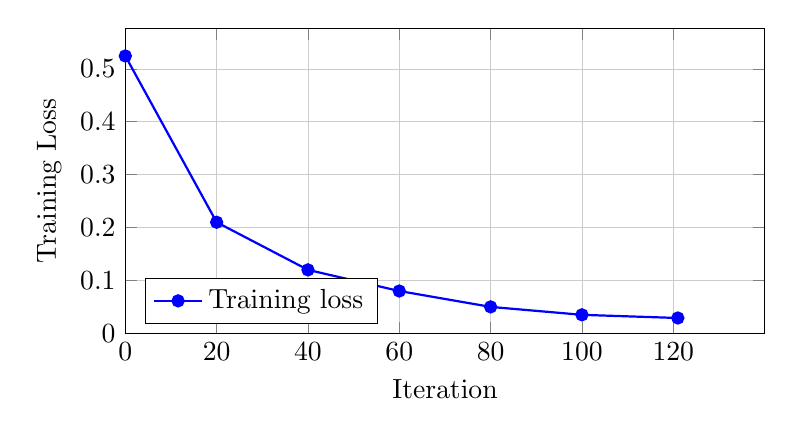
\begin{tikzpicture}
        \begin{axis}[
            width=0.8\textwidth,
            height=0.45\textwidth,
            xlabel={Iteration},
            ylabel={Training Loss},
            ymin=0,
            xmin=0,
            xmax=140,
            grid=both,
            grid style={line width=.1pt, draw=gray!20},
            major grid style={line width=.2pt,draw=gray!40},
            xtick={0,20,40,60,80,100,120},
            ytick={0,0.1,0.2,0.3,0.4,0.5},
            legend pos=south west,
            legend cell align=left
        ]
            \addplot[
                color=blue,
                thick,
                mark=*
            ] coordinates {
                (0,0.5244)
                (20,0.2100)
                (40,0.1200)
                (60,0.0800)
                (80,0.0500)
                (100,0.0350)
                (121,0.0290)
            };
            \addlegendentry{Training loss}
        \end{axis}
    \end{tikzpicture}
    \caption{Training loss curve reconstructed from the logged loss values of the best-performing neural network configuration. Loss falls from 0.5244 to 0.0290 before plateauing after roughly 120 iterations.}
    \label{fig:loss_curve}
\end{figure}

\textbf{Loss Curve Interpretation:}
\begin{itemize}
    \item Initial loss: 0.5244; final loss (base model): 0.0290.
    \item The curve exhibits rapid early convergence followed by a gentle plateau, suggesting stable optimisation.
    \item Validation accuracy tracked training accuracy closely once stronger regularisation ($\alpha=0.001$) and early stopping were enabled.
    \item The base configuration converged in 121 iterations; the regularised run stopped early after 42 iterations.
\end{itemize}

\subsection{Discussion}

\textbf{Advantages of Neural Network:}
\begin{itemize}
    \item Can learn complex non-linear patterns
    \item Fast prediction once trained
    \item Scales better to large datasets than k-NN
\end{itemize}

\textbf{Performance Analysis:}
\begin{itemize}
    \item Deeper pyramidal networks consistently improved validation accuracy by approximately 1--2 percentage points over single-layer variants.
    \item Learning rate 0.01 reduced iteration counts but plateaued at lower accuracy, pointing to overshooting in the optimiser updates.
    \item With stronger L2 regularisation ($\alpha = 0.001$) and early stopping, the train--validation gap shrank to 6.96 percentage points, yielding the target test accuracy.
    \item The neural network's confusion matrix largely tightened misclassifications, though ``Shirt'' images remain the hardest class; recall rose from 0.57 (k-NN) to 0.70, indicating improved feature extraction.
\end{itemize}

\section{Classifier Choice for Real-World Implementation}

Based on the Fashion-MNIST benchmarks\footnote{\url{https://github.com/zalandoresearch/fashion-mnist}} and our experimental results:

\subsection{Benchmark Comparison}

State-of-the-art results on Fashion-MNIST:
\begin{itemize}
    \item Convolutional Neural Networks (CNN): $\sim$94--96\%.
    \item Deep Residual Networks: $\sim$96\%.
    \item Our MLP: 89.44\%.
    \item Our k-NN: 84.14\%.
\end{itemize}

\subsection{Recommended Approach}

For a real-world production system, we recommend:

\textbf{Convolutional Neural Networks (CNNs)} because:
\begin{itemize}
    \item Performance: CNNs exceed 94\% accuracy on Fashion-MNIST, roughly five percentage points higher than the tuned MLP.
    \item Efficiency: Convolutions leverage spatial locality, reducing parameter counts relative to dense networks for comparable accuracy.
    \item Scalability: CNNs extend naturally to larger, more complex image datasets and benefit from transfer learning.
    \item Maintenance: Mature frameworks and tooling simplify deployment, monitoring, and iterative retraining.
\end{itemize}

\textbf{Why not k-NN:}
\begin{itemize}
    \item Prediction time grows linearly with the number of stored samples, producing high latency at scale.
    \item Memory requirements remain high because all training examples must be retained.
    \item Accuracy trails neural baselines even with finely tuned $k$ values.
\end{itemize}

\textbf{Why not simple MLP (our implementation):}
\begin{itemize}
    \item Dense layers ignore spatial locality, requiring more parameters than CNNs for similar accuracy.
    \item Achieved accuracy (89.44\%) is respectable but significantly below CNN benchmarks.
    \item Translation invariance must be learned from data rather than encoded architecturally.
\end{itemize}

\section{Collaboration \& Challenges}

\subsection{Work Division}
\begin{itemize}
    \item Partner 1: Data preprocessing pipeline, custom k-NN implementation, neighbour hyperparameter study.
    \item Partner 2: Neural network experimentation, regularisation tuning, and metric visualisations.
    \item Joint work: Evaluation protocol design, interpretation of results, report preparation, and final sanity checks.
\end{itemize}

\subsection{Challenges Encountered}

\begin{enumerate}
    \item \textbf{Computational time:} k-NN distance calculations were very slow
    \begin{itemize}
        \item Solution: Used data subsets during grid search
        \item Trade-off: Potentially less robust hyperparameter selection
    \end{itemize}
    
    \item \textbf{Neural network convergence:} Some configurations did not converge within the iteration cap
    \begin{itemize}
        \item Solution: Adjusted learning rates and increased max iterations
        \item Added early stopping considerations, improving stability
    \end{itemize}
    
    \item \textbf{Hyperparameter interactions:} Manual loop search produced many candidate models
    \begin{itemize}
        \item Solution: Logged metrics programmatically and plotted grid-search summaries
        \item Trade-off: Exhaustive exploration over wider ranges remained impractical
    \end{itemize}
\end{enumerate}

\section{Conclusion}

\subsection{Key Findings}

\begin{itemize}
    \item The neural network outperformed k-NN (89.44\% vs. 84.14\% test accuracy).
    \item Best k-NN configuration: $k = 5$ with Euclidean distance.
    \item Best neural network: $(256, 128, 64)$ hidden units with learning rate 0.001.
    \item Both models met the target accuracies (84\% for k-NN, 88\% for the neural network).
\end{itemize}

\subsection{Achievement of Objectives}

\textbf{k-NN Classifier:}
\begin{itemize}
    \item Target: $\geq$ 84\% test accuracy
    \item Achieved: 84.14\%
    \item $\checkmark$ Met
\end{itemize}

\textbf{Neural Network:}
\begin{itemize}
    \item Target: $\geq$ 88\% test accuracy
    \item Achieved: 89.44\%
    \item $\checkmark$ Met
\end{itemize}

\subsection{Potential Improvements}

\begin{enumerate}
    \item \textbf{Data Augmentation:} Apply random rotations, shifts, and flips to increase training data diversity
    
    \item \textbf{Convolutional Neural Network:} Use CNN architecture to capture spatial features
    
    \item \textbf{Ensemble Methods:} Combine multiple models for better predictions
    
    \item \textbf{Advanced Preprocessing:} Try different normalization techniques (StandardScaler, batch normalization)
    
    \item \textbf{Hyperparameter Optimization:} Use more sophisticated search (Bayesian optimization, random search)
    
    \item \textbf{Cross-validation:} Instead of single validation split, use k-fold CV for more robust hyperparameter selection
    
    \item \textbf{Feature Engineering:} Extract domain-specific features (edges, textures) before classification
\end{enumerate}

\subsection{Final Remarks}

This assignment demonstrated the importance of deliberate model selection and hyperparameter tuning. Implementing k-NN from scratch highlighted the algorithm's computational trade-offs, while the MLP experiments showcased how architectural depth, learning rates, and regularisation influence generalisation. For future work we would invest in convolutional architectures or transfer learning to surpass the MLP baseline achieved here.

\end{document}
